
\documentclass[a4paper,10pt]{article}
%\usepackage{fullpage}
\usepackage[utf8]{inputenc}
\usepackage[swedish]{babel}
\usepackage{todonotes}

\usepackage{url}
\usepackage{titlesec}

%\usepackage{algorithmicx}
\usepackage{algorithm}
\usepackage{algpseudocode}
\algnewcommand{\LineComment}[1]{\State \(\triangleright\) #1}
\algnewcommand{\Continue}{\textbf{continue}}
\algnewcommand{\Vspace}{\item[]}
\algnewcommand{\To}{\textbf{to}~}

\usepackage{mathtools}
\DeclarePairedDelimiter\ceil{\lceil}{\rceil}
\DeclarePairedDelimiter\floor{\lfloor}{\rfloor}
\newcommand{\addeq}{\mathrel{+}=}
\newcommand{\subeq}{\mathrel{-}=}
\newcommand{\unioneq}{\mathrel{\cup}=}
\newcommand{\addadd}{\mathrel{++}}
\newcommand{\subsub}{\mathrel{--}}

\usepackage{framed}

%\usepackage[section]{placeins}

\usepackage{graphicx}
\usepackage{caption}
\usepackage{subcaption}

\usepackage{amsmath}

\title{{\small 1TE717 Digitalteknik och Elektronik, Projekt} \\ \textbf{Digital överföring av ljudvågor via RF-radio}}

\author{Bj{\"o}rn Forsberg \and Sven Lundgren \and Jonathan Sharyari}
%\textwidth 5.5in 
%\oddsidemargin 0.5in 

\begin{document}

\maketitle

\abstract

Denna rapport beskriver en implementation av ett system för digital 
överföring av ljud som en del av det projekt som ingår i kursen Digitalteknik 
och Elektronik (1TE717). Systemet använder en mikrofon för att fånga upp 
ljudvågor, vilka sedan konverteras till en digital signal och sänds via radio 
till en mottagare. Mottagaren konverterar tillbaka signalen till en analog 
representation som sedan kan spelas upp på en högtalare. Den digitala 
överföringen minskar risken för störningar, då risken att en etta och nolla ska 
flippa är mindre än risken för störningar på en analog signal.

Vid enklare tester visar sig systemet kapabelt att föra över mycket exakta 
signaler från sändare till mottagare. Det är dock mycket känsligt för att hamna
i otakt, i det att överföringen inte har någon tydlig början och slut. I och med
detta måste mottagaren manuellt synkronisera signalen, om så endast en gång vid 
systemstart. Slutligen använder denna implementation en delad klocksignal mellan 
sändare och mottagare, vilket reducerar den praktiska användbarheten av 
systemet. Det lämnas till framtida arbete att implementera en distribuerad 
klockning av systemet.

\section{Inledning}

Att överföra ljud elektroniskt mellan två punkter är ett av de största 
genombrotten inom kommunikation. Det har tillåtit vänner och familjer  att hålla 
kontakten över stora avstånd, gjort det möjligt för stater att kommunicera i 
realtid.

Traditionellt sett har ljudsignalerna överförts från vibrationer i luften till
förändringar i elektrisk spänning med hjälp av en mikrofon. I denna analoga 
representation, motsvaras tryckförändringar i luften direkt av 
spänningsförändringar i mikrofonens utsignal. På motsvarande sätt överförs de
elektriska signalerna tillbaka till ljudsignaler via en högtalare, genom att 
framkalla tryckförändringar i luften motsvarande spänningsförändringarna i
den elektriska signalen.

I dag sker allt större delar av världens informationsöverföring i digital form, 
där informationen istället uttrycks i sekvenser av höga (t.ex. $5V$) och låga
(t.ex. $0V$) signaler. För att representera ljudvågor digitalt behöver således 
tryckförändringarna i luften översättas till diskreta värden, som kan 
representeras av ett tal.
Exempelvis kan intervallet $[u^{min}, u^{max}]$ delas upp i $n$ diskreta 
delintervall, var och en representerad av ett binärt tal. Ju högre man väljer
$n$, desto fler bitar behövs för att representera alla delintervall, men ju
bättre approximeras den analoga signalen av den digitala. Antalet intervall som 
kan representeras ges av uttrycket $n = 2^b$ där $b > 0$ och ger antalet bitar 
som används för att uttrycka värdet. Elektriska komponenter som översätter 
analoga spänningar till dess digitala representation kallas 
analog-till-digital-omvandlare (AD-omvandlare, ADC). 
För att återföra den digitala signalen till sin analoga form används en
digital-till-analog-omvandlare (DA-omvandlare, DAC), vars funktion är
inversen av ADC:ns. 

Denna rapport presenterar ett projekt om $4 hp$, i vilket ett 
ljudöverföringssystem implementeras. Med hjälp av en mikrofon fångas en 
ljudsignal upp, omvandlas till en digital representation, varpå denna digitala 
representation överförs seriellt via radiovågor till en mottagare. Mottagaren 
omvandlar i sin tur den digitala representationen tillbaka till en analog signal 
som kan omvandlas till ljud av en högtalare.

Att gå igenom dessa steg för att omvandla en analog signal till en digital, för
att sedan direkt återföra den till den analoga representationen kan låta 
onödigt, men motiveras utav den lägre störningsrisken i digital överföring. 
Detta eftersom att en störning på en analog signal överlagras in i signalen, och
det är kostsamt att rensa ut dessa störningar. I motsats kommer en störning på
en digital signal i normalfallet inte påverka informationen i signalen, eftersom
att störningen måste vara mycket stor för att signalens betydelse ska skifta
mellan logiskt hög till låg eller vice versa.


\section{Genomförande}

Systemet implementeras i tre separata delar där varje del utför en avgränsad 
uppgift inom systemet. Den första delen hanterar ljudupptagning, vilket sker med
hjälp av en vanlig mikrofon. De två senare delarna implementerar sändare
respektive mottagare för den digitaliserade ljudsignalen. En översikt av 
systemet presenteras i Figur \ref{fig:sysoversikt}.

\begin{figure}[h]
    \centering
    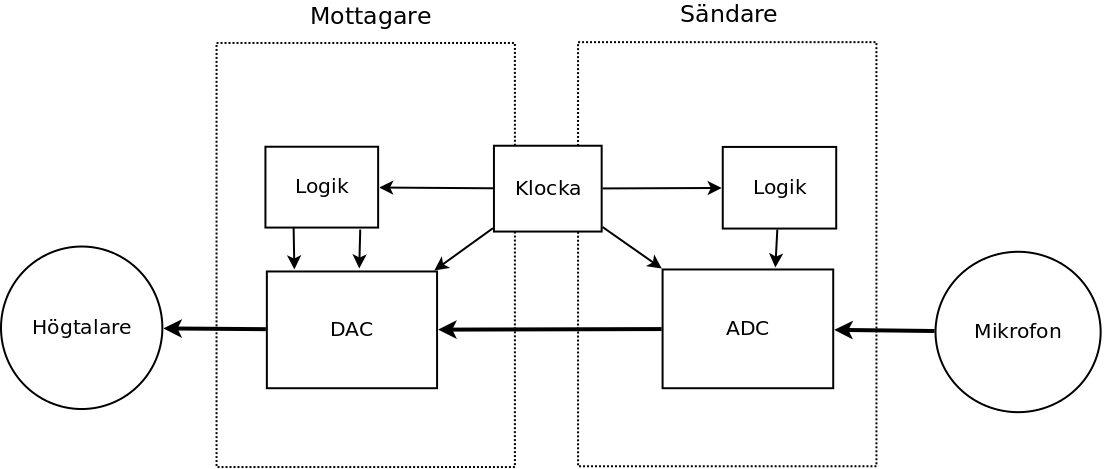
\includegraphics[width=\textwidth]{sysoversikt.png}
    \caption{En översiktlig vy över det implementerade systemet.}
    \label{fig:sysoversikt}
\end{figure}

Sändar- och mottagardelarna styrs av ett enkelt kombinatoriskt nät som ger 
styrsignalerna till ADC och DAC. Ut- respektive insignalerna till ADC och DAC
förs sedan över via radio. De komponenter som använts presenteras i Tabell 
\ref{tab:komponenter}. 

Resterande del av denna sektion är uppdelad i tre undersektioner. Den första beskriver implementationen av mikrofonkretsen, varefter den andra beskriver omvandlingen mellan digitala och analoga representationer, samt överföringen av denna information. Slutligen beskrivs hur de synkrona komponenterna klockas. För att spela upp utsignalen användes en färdig högtalare, och denna komponent beskrivs därför inte närmre.

\begin{table}[h]
    \centering
    \begin{tabular}{|l|l|}
    \hline
    1 st & Texas Instruments ADS7816P, 12-bit serial ADC \\
    1 st & Texas Instruments DAC7611P, 12-bit serial DAC \\
    1 st & Seriell radiosändare och mottagare \\
    1 st & Mikrofon KEEG1538WB-100LB \\
    2 st & 4-bitars räknare \\
    1 st & 4-vägs AND-grind\\
    1 st & 2-vägs AND-grind \\
    1 st & 2-vägs XOR-grind \\
    1 st & NOT-grind \\
	 & Funktionsgenerator \\
    \hline
    \end{tabular}
    
    \caption{Komponenterna som använts för att implementera systemet.}
    \label{tab:komponenter}

\end{table}

\subsection{Mikrofon}

Med hjälp av en enkel mikrofon förs en ljudsignal in i systemet. 
I databladet för mikrofonen hittas den grundläggande krets som krävs för att 
omvandla vibrationerna i mikrofonen till en analog elektrisk signal, se Figur 
\ref{fig:mikrofon}.

\begin{figure}[h]
    \centering
    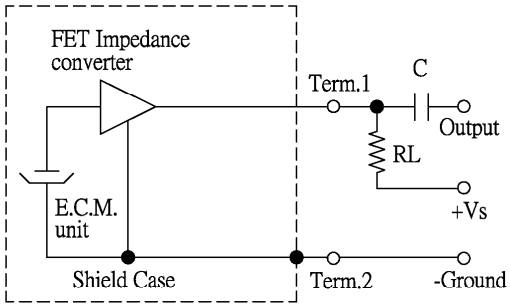
\includegraphics[width=0.6\textwidth]{mik.jpg}
    \caption{Krets för att få ut den analoga elektriska signal som representerar
	     vibrationerna som tas upp av mikrofonen. Hämtat från mikrofonens
	     datablad.}
    \label{fig:mikrofon}
\end{figure}

Denna krets skapar en mycket svag sinusformad signal i storleksordningen 
$\pm 10 mV$. För att digitalisera signalen behöver den förstärkas för att 
spänningsnivåerna i signalen ska spridas över ett större intervall, vilket ger 
större inbördes skillnader mellan de diskreta spänningsnivåer som uppmäts av 
AD-omvandlaren. För detta används två operationsförstärkare, en för att 
förstärka signalen till $\pm 2.5 V$, och den andra för att lyfta signalens 
effektivvärde från $0$ till $2.5 V$. Dessa två operationer optimerar signalen
för att de uppmätta värdena ska hamna inom AD-omvandlarens referensinterval
$[0,5V]$.

\subsection{Digital överföring}

För att omvandla den analoga ljudsignalen till en digital signal, och sända den 
trådlöst används enkla $433 MHz$-sändare och -mottagare. Dessa komponenter
beter sig på samma sätt som en kabelbunden ledare, i det att den spänning i 
intervallet $[0, 5V]$ som läggs på sändarens datapin återges på mottagarens
motsvarighet. Av denna anledning beskrivs inte överföringen som sådan närmre,
utan de två följande undersektionerna presenterar hur data kodas och avkodas
i sändare respektive mottagare.


\subsubsection{Sändare}

Den mest centrala komponenten i sändaren är ADC:n, som konverterar den analoga
signalen från mikrofonen till en 12-bitars digital signal som sedan sänds över
radio.

Det finns ett mycket stort utbud av integrerade kretsar för ADC:er på marknaden,
med flera inbördes olika egenskaper. Det första att ta hänsyn till vid valet av
ADC är seriell eller parallel utsignal. Eftersom att utsignalen skickas över 
radio som en seriell signal är valet av seriell ADC uppenbart. För seriella 
komponenter finns sedan åtskilliga val vad gäller protokoll som kontrollerar när
och hur data skickas ut från komponenten. I detta fall föll valet på en 
SPI-bestyckad ADC, eftersom att SPI är ett förhållandevis enkelt protokoll, och
därmed lätt att kontrollera med hjälp av enkla kombinatoriska nät, i motsats 
till mer avancerade protokoll där en mikrokontroller är mer eller mindre
nödvändig. Eftersom att SPI definerar hur data förs över rent fysiskt mycket
hårdare än det definerar vilken data som skickas, finns det flera olika 
implementationer av dataprotokollet.

Det slutgiltiga valet föll på $ADS7816P$, en SPI-bestyckad 12-bitars 
ADC med ett mycket enkelt dataprotokoll, se Figur \ref{fig:adcproto}, vilken 
därför kräver ett mycket enkelt kombinatoriskt när för att styra. ADC:n använder 
fyra klockcykler för att sampla en inkommande signal, och 12 cycler för att
seriellt sända ut dess digitala representation. Sampling påbörjas då 
styrsignalen \emph{CS} (Chip Select) går från hög till låg. Detta resulterar i 
sanningstabellen i tabell \ref{tab:adc} och det motsvarande kombinatoriska nätet 
i Figur \ref{fig:adccircuit}.

\begin{figure}[h]
\centering
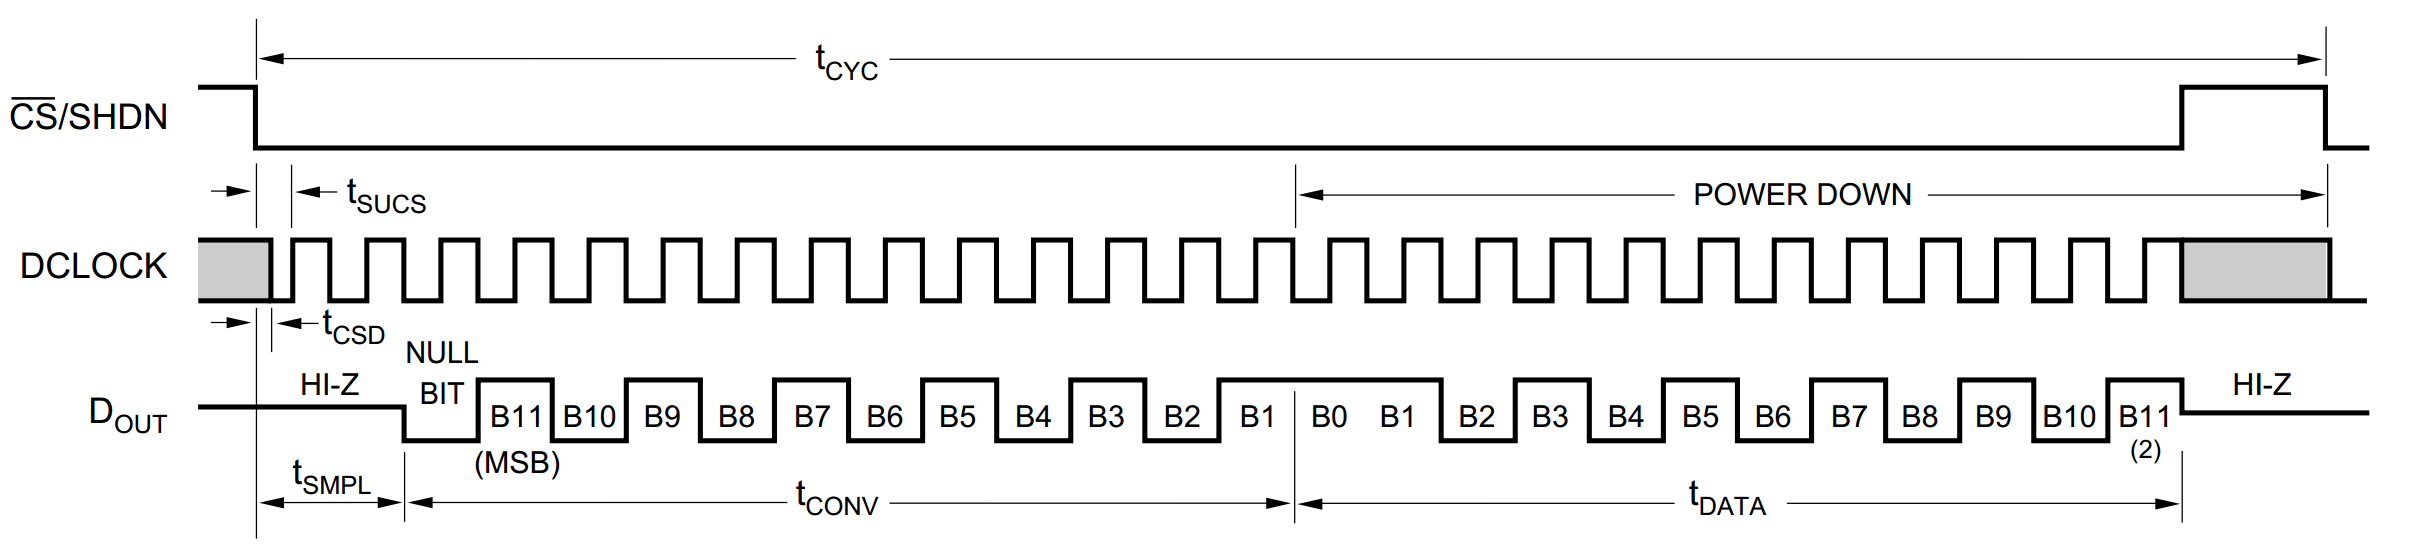
\includegraphics[width=\textwidth]{adcdiagram.png}
\caption{Dataprotokoll för AD-omvandlaren, hämtat från dess datablad.}
\label{fig:adcproto}
\end{figure}

\begin{table}[h]
\centering
\begin{tabular}{| c c c c || c |}
\hline
$x_3$ & $x_2$ & $x_1$ & $x_0$ & $cs$ \\\hline
0 & 0 & 0 & 0 & 0 \\
0 & 0 & 0 & 1 & 0 \\
0 & 0 & 1 & 0 & 0 \\
0 & 0 & 1 & 1 & 0 \\
0 & 1 & 0 & 0 & 0 \\
0 & 1 & 0 & 1 & 0 \\
0 & 1 & 1 & 0 & 0 \\
0 & 1 & 1 & 1 & 0 \\
1 & 0 & 0 & 0 & 0 \\
1 & 0 & 0 & 1 & 0 \\
1 & 0 & 1 & 0 & 0 \\
1 & 0 & 1 & 1 & 0 \\
1 & 1 & 0 & 0 & 0 \\
1 & 1 & 0 & 1 & 0 \\
1 & 1 & 1 & 0 & 0 \\
1 & 1 & 1 & 1 & 1 \\
\hline
\end{tabular}

$cs$ = $x_3 \wedge x_2 \wedge x_1 \wedge x_0$

\caption{Sanningstabell för styrsignaler för AD-omvandlaren.}
\label{tab:adc}
\end{table}

\begin{figure}[h]
\centering
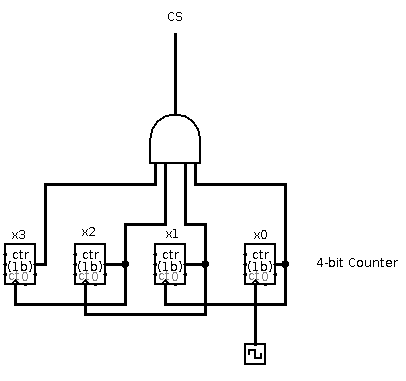
\includegraphics[width=0.6\textwidth]{adccircuit.png}
\caption{Kopplingsschema för styrsignaler för AD-omvandlaren.}
\label{fig:adccircuit}
\end{figure}


\subsubsection{Mottagare}

Liksom för sändaren är det konverteringen mellan analog och digital data som
är den centrala funktionen i mottagaren. I detta fall är det den digitala 
signalen som mottages över radio som ska konverteras tillbaka till en analog
signal som kan tolkas av högtalaren.

Liksom för valet av ADC i sändaren finns det en stor variation av tillgängliga 
DAC:ar på marknaden. Eftersom att mottagaren ska vara kompatibel med sändaren
är även denna 12-bitars seriell, och liksom ADC:n föll protokollvalet på SPI. 
Även här var en enkel implementation av SPI avgörande och därför valdes 
slutligen $DAC7611P$ för mottagarens DA-omvandling. 

Denna DAC kräver förutom $CS$-signalen även en $LD$-signal för att ladda in data
i registret, se protokollet i Figur \ref{fig:dacprotocol}. Detta ger ett något 
mer komplicerat grindnät än på sändarsidan, och 3 grindar krävs för att 
producera insignalerna. Grindnätet baseras på sanningstabellen i Tabell 
\ref{tab:dac}, och presenteras i Figur 
\ref{fig:daccircuit}.

\begin{figure}[h]
\centering
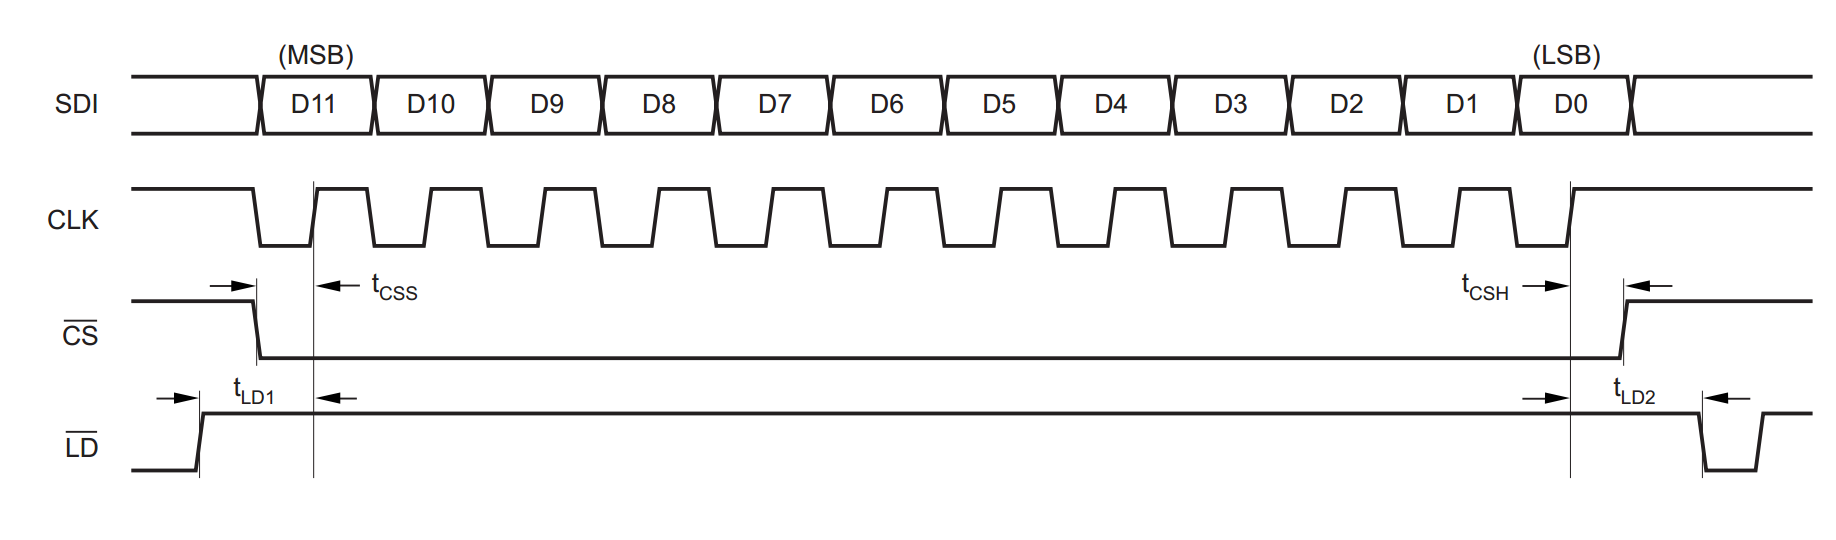
\includegraphics[width=\textwidth]{dacdiagram.png}
\caption{Dataprotokoll för DA-omvandlaren, hämtat från dess datablad.}
\label{fig:dacprotocol}
\end{figure}

\begin{table}[h]
\centering
\begin{tabular}{|c c c c || c c |}
\hline
$x_3$ & $x_2$ & $x_1$ & $x_0$ & $cs$ & $ld$ \\\hline
0 & 0 & 0 & 0 & 0 & 1 \\
0 & 0 & 0 & 1 & 0 & 1 \\
0 & 0 & 1 & 0 & 0 & 1 \\
0 & 0 & 1 & 1 & 0 & 1 \\
0 & 1 & 0 & 0 & 0 & 1 \\
0 & 1 & 0 & 1 & 0 & 1 \\
0 & 1 & 1 & 0 & 0 & 1 \\
0 & 1 & 1 & 1 & 0 & 1 \\
1 & 0 & 0 & 0 & 0 & 1 \\
1 & 0 & 0 & 1 & 0 & 1 \\
1 & 0 & 1 & 0 & 0 & 1 \\
1 & 0 & 1 & 1 & 0 & 1 \\
1 & 1 & 0 & 0 & 1 & 1 \\
1 & 1 & 0 & 1 & 1 & 0 \\
1 & 1 & 1 & 0 & 1 & 0 \\
1 & 1 & 1 & 1 & 1 & 1 \\
\hline
\end{tabular}

$cs$ = $x_3 \wedge x_2$

$ld$ = $x3 \wedge x_2 \wedge (x_1 \oplus x_0)$

\caption{Sanningstabell för styrsignaler för DA-omvandlaren.}
\label{tab:dac}
\end{table}

\begin{figure}[h]
\centering
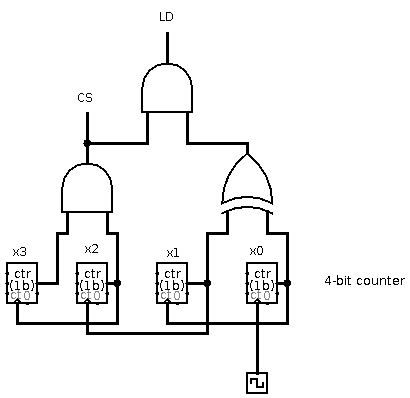
\includegraphics[width=0.6\textwidth]{daccircuit.png}
\caption{Kopplingsschema för styrsignaler för DA-omvandlaren.}
\label{fig:daccircuit}
\end{figure}




\subsection{Klocka och klockpulser}

Systemet utnyttjar flera synkrona integrerade kretsar som kräver en
klockpuls. Klockpulsen styr kretsarnas arbetstakt, och således betyder en hög 
klockpuls att systemet arbetar i en högre takt. Klockpulsen är i detta system 
input till de två integrerade kretsar som agerar sändare och mottagare, där den 
styr hastigheten på kretsernas räknarkomponent. I figur \ref{fig:adccircuit} och 
\ref{fig:daccircuit} kan observeras att var sextonde klockpuls ger så kallad 
\textit{chip select} signal i båda kretsarna, vilket innebär att AD- eller 
DA-omvandlaren ska börja sampla ett nytt värde. Detta i sin tur innebär att 
systemets verkliga arbetstakt gällande konvertering mellan analoga och digitala 
ljudsignaler är $\frac{1}{16}$ av den givna klockfrekvensen.

Konvertering av tidskontinuerliga signaler till tidsdiskreta signaler beskrivs 
av \textit{Nyquist-Shannons samplingsteorem} \cite{sampling}. Teoremet säger i 
grova drag att för att undvika fel vid diskret sampling av tidskontinuerliga 
signaler bör samplingstakten vara minst dubbla signalens bandbredd. I detta 
projekt antas en bandbredd på $4KHz$ täcka det frekvensband som krävs för att 
fånga upp alla nyanser av mänskligt tal. Samplingsfrekvensen måste då vara 
minst $8KHz$ vilket i sin tur innebär att systemets klockfrekvens måste vara 
minst $16 \times 8KHz = 128KHz$.

Då en snabb klockpuls måste ges till hela systemet för att garantera tillräcklig 
kvalitet på ljudsignalen krävs att de komponenter som ingår i systemet tål denna 
höga klockpuls. Dessa komponenter inkluderar räknare, ADC och DAC.

Eftersom att klocksynkronisering är ett stort och välkänt problem, har det 
utelämnats i detta projekt, och klockpulsen delas således av sändare och 
mottagare i den nuvarande implementationen. 


\section{Resultat}

Det implementerade systemet klarar av att relativt störningsfritt överföra 
ljudsignaler mellan sändare och mottagare. Då en gemensam klocka används
krävs ingen synkronisering under körning, däremot krävs initial synkronisering
då komponenterna aktiveras vid olika tidpunkter. För att initialt 
synkronisera sändare och mottagare läggs en hög resetsignal till DAC:n 
med en vanlig tryckknapp. Sannolikheten att komponenterna är synkroniserade
efter en sådan signal är $\frac{1}{16}$, och proceduren upprepas således 
till dess att ljudåtergivningen är korrekt. 

I Figur \ref{oscilloskop} kan den ursprungliga analoga ljudsignalen (efter förstärkning) ses jämte den återskapade analoga signalen efter att den digitala
signalen avkodats. Det framgår tydligt hur den återskapade signalen är uppbyggd av ett antal diskreta värden, en effekt som avtar vid högre klockfrekvenser.

\begin{figure}[h]
\centering
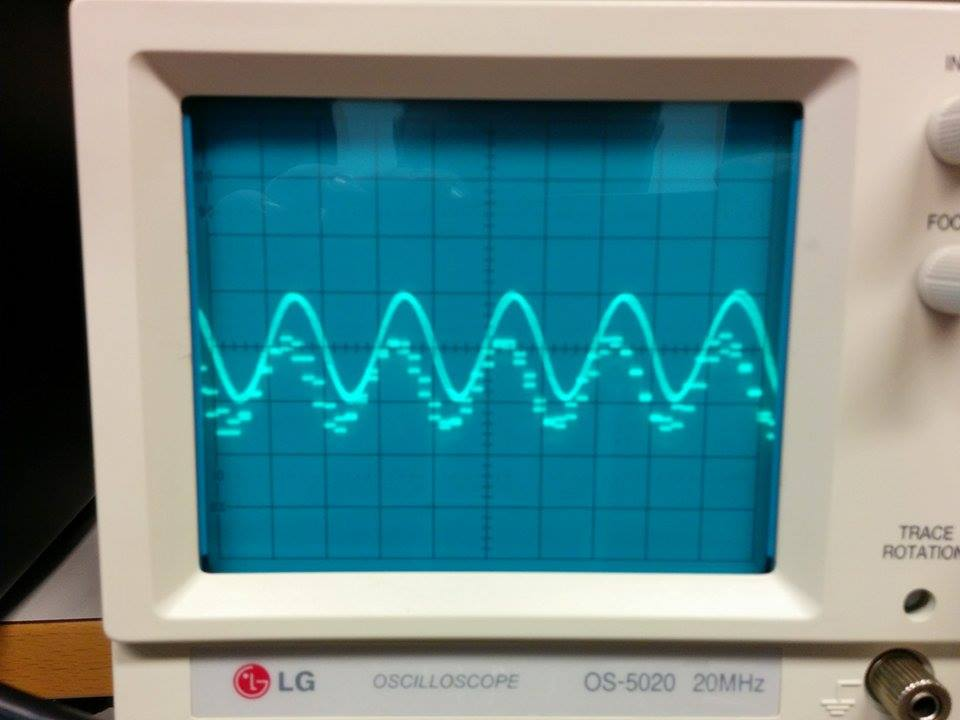
\includegraphics[width=0.84\textwidth]{oscilloskop.jpg}
\caption{Analoga signaler före och efter digitalisering. Den kontinuerliga 
         kurvan utgör den ursprungliga signalen och den streckade kurvan den 
	 återskapade signalen.}
\label{oscilloskop}
\end{figure}


\section{Diskussion}
\subsection{Störningar}
De störningar som uppstår har främst två orsaker. Vid trådlös överföring finns 
alltid risken att data korrumperas eller försvinner, en risk som ökar med 
avståndet mellan sändare och mottagare. Utöver detta så används en samplingstakt 
på $128 KHz$, med vilken frekvenser upp till $4 KHz$ kan återskapas. Eftersom 
att mikrofonen även fångar upp högre frekvenser innebär detta att dessa 
frekvenser feltolkas vid sampling och tillför en mindre störning till signalen. 
Problemet avhjälps enkelt med ett lågpassfilter som filtrerar bort högre 
frekvenser från den analoga signalen innan den når AD-omvandlaren.

\subsection{Synkronisering}
\label{synkronisering}

Varaktig synkronisering med distribuerade klockor är generellt ett svårt problem 
att lösa. Det är dock möjligt att implementera enklare lösningar om man är
villig att acceptera en viss felfrekvens. I fallet ljudöverföring är 
feltoleransen relativt hög, och det är därför möjligt att implementera 
förenklade synkroniseringsmekanismer. Ett sätt att göra detta är att utnyttja 
det faktum att både ADC och DAC använder 16 klockcykler för att överföra 12 
bitar data. Under de fyra klockcykler som ADC:n inte skickar data skickas 
istället ettor (höga signaler). Digitalomvandlaren tar då emot fyra ettor innan 
den relevanta informationen. Denna representationsinvariant kan utnyttjas för
synkronisering, i det att DA-omvandlarens \emph{LD}-signal sätts till hög vid 
den tredje mottagna ettan, varpå \emph{CS}-signalen sätts till låg vid den 
fjärde, varvid data läses in. Denna lösning skulle dock innebära att i de fall
den binära representationen av den siffra i den digitala signalen som 
för tillfället sänds innehåller fyra efter varandra följande ettor skulle detta feltolkas som synkroniseringssignal, och systemet skulle temporärt vara osynkroniserat.

\begin{thebibliography}{hejhej}

\bibitem{sampling}
    {Cand{\`e}s, Emmanuel J and Wakin, Michael B,
    \emph{An introduction to compressive sampling},
    Signal Processing Magazine, IEEE,
    volume 25,
    number 2,
    pages 21-30,
    2008.
}
\end{thebibliography}


\end{document}
